\begin{problem}{Laser Beam}{stdin}{stdout}{5 seconds}{64 megabytes}

There is an equilateral triangle consist of 3 mirrors. There is a tiny slit in the corners of the triangle, which can let a laser beam pass through.

\begin{center}
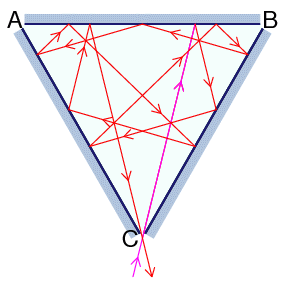
\includegraphics{figure.png}
\end{center}


We label the 3 slits as $A$, $B$ and $C$. There only exists two ways (see the picture above) make a laser beam enter our triangle though $C$, reflects 11 times in ther triangle, and exit from the triangle though $C$. The 2 ways are symmetry.

Here is the question for you, our great programmer. How many ways we can make a laser beam enter the triangle though $C$ and exit though $C$, and the beam reflects $n$ times in the triangle? e.g. there are 80840 ways when $n$ is 1000001.


\InputFile
The first line contains a number $T$.($1\leq T\leq 100$)
Then the following $T$ line each line contains a number $n$.($1\leq n\leq 10^7$)

\OutputFile
For each $n$, print the corresponding result.

\Examples

\begin{example}
\exmp{10
2
5
7
11
13
17
19
23
29
31
}{0
0
2
2
2
0
4
4
2
6
}%
\end{example}

\end{problem}
